\documentclass[twoside]{book}

% Packages required by doxygen
\usepackage{fixltx2e}
\usepackage{calc}
\usepackage{doxygen}
\usepackage[export]{adjustbox} % also loads graphicx
\usepackage{graphicx}
\usepackage[utf8]{inputenc}
\usepackage{makeidx}
\usepackage{multicol}
\usepackage{multirow}
\PassOptionsToPackage{warn}{textcomp}
\usepackage{textcomp}
\usepackage[nointegrals]{wasysym}
\usepackage[table]{xcolor}

% Font selection
\usepackage[T1]{fontenc}
\usepackage[scaled=.90]{helvet}
\usepackage{courier}
\usepackage{amssymb}
\usepackage{sectsty}
\renewcommand{\familydefault}{\sfdefault}
\allsectionsfont{%
  \fontseries{bc}\selectfont%
  \color{darkgray}%
}
\renewcommand{\DoxyLabelFont}{%
  \fontseries{bc}\selectfont%
  \color{darkgray}%
}
\newcommand{\+}{\discretionary{\mbox{\scriptsize$\hookleftarrow$}}{}{}}

% Page & text layout
\usepackage{geometry}
\geometry{%
  a4paper,%
  top=2.5cm,%
  bottom=2.5cm,%
  left=2.5cm,%
  right=2.5cm%
}
\tolerance=750
\hfuzz=15pt
\hbadness=750
\setlength{\emergencystretch}{15pt}
\setlength{\parindent}{0cm}
\setlength{\parskip}{3ex plus 2ex minus 2ex}
\makeatletter
\renewcommand{\paragraph}{%
  \@startsection{paragraph}{4}{0ex}{-1.0ex}{1.0ex}{%
    \normalfont\normalsize\bfseries\SS@parafont%
  }%
}
\renewcommand{\subparagraph}{%
  \@startsection{subparagraph}{5}{0ex}{-1.0ex}{1.0ex}{%
    \normalfont\normalsize\bfseries\SS@subparafont%
  }%
}
\makeatother

% Headers & footers
\usepackage{fancyhdr}
\pagestyle{fancyplain}
\fancyhead[LE]{\fancyplain{}{\bfseries\thepage}}
\fancyhead[CE]{\fancyplain{}{}}
\fancyhead[RE]{\fancyplain{}{\bfseries\leftmark}}
\fancyhead[LO]{\fancyplain{}{\bfseries\rightmark}}
\fancyhead[CO]{\fancyplain{}{}}
\fancyhead[RO]{\fancyplain{}{\bfseries\thepage}}
\fancyfoot[LE]{\fancyplain{}{}}
\fancyfoot[CE]{\fancyplain{}{}}
\fancyfoot[RE]{\fancyplain{}{\bfseries\scriptsize Generated by Doxygen }}
\fancyfoot[LO]{\fancyplain{}{\bfseries\scriptsize Generated by Doxygen }}
\fancyfoot[CO]{\fancyplain{}{}}
\fancyfoot[RO]{\fancyplain{}{}}
\renewcommand{\footrulewidth}{0.4pt}
\renewcommand{\chaptermark}[1]{%
  \markboth{#1}{}%
}
\renewcommand{\sectionmark}[1]{%
  \markright{\thesection\ #1}%
}

% Indices & bibliography
\usepackage{natbib}
\usepackage[titles]{tocloft}
\setcounter{tocdepth}{3}
\setcounter{secnumdepth}{5}
\makeindex

% Hyperlinks (required, but should be loaded last)
\usepackage{ifpdf}
\ifpdf
  \usepackage[pdftex,pagebackref=true]{hyperref}
\else
  \usepackage[ps2pdf,pagebackref=true]{hyperref}
\fi
\hypersetup{%
  colorlinks=true,%
  linkcolor=blue,%
  citecolor=blue,%
  unicode%
}

% Custom commands
\newcommand{\clearemptydoublepage}{%
  \newpage{\pagestyle{empty}\cleardoublepage}%
}

\usepackage{caption}
\captionsetup{labelsep=space,justification=centering,font={bf},singlelinecheck=off,skip=4pt,position=top}

%===== C O N T E N T S =====

\begin{document}

% Titlepage & ToC
\hypersetup{pageanchor=false,
             bookmarksnumbered=true,
             pdfencoding=unicode
            }
\pagenumbering{alph}
\begin{titlepage}
\vspace*{7cm}
\begin{center}%
{\Large 4D Chess }\\
\vspace*{1cm}
{\large Generated by Doxygen 1.8.13}\\
\end{center}
\end{titlepage}
\clearemptydoublepage
\pagenumbering{roman}
\tableofcontents
\clearemptydoublepage
\pagenumbering{arabic}
\hypersetup{pageanchor=true}

%--- Begin generated contents ---
\chapter{Hierarchical Index}
\section{Class Hierarchy}
This inheritance list is sorted roughly, but not completely, alphabetically\+:\begin{DoxyCompactList}
\item \contentsline{section}{Flats\+Data}{\pageref{struct_flats_data}}{}
\item I\+Event\+Receiver\begin{DoxyCompactList}
\item \contentsline{section}{My\+Event\+Receiver}{\pageref{class_my_event_receiver}}{}
\end{DoxyCompactList}
\item \contentsline{section}{Pices\+Pos}{\pageref{struct_pices_pos}}{}
\item Q\+Object\begin{DoxyCompactList}
\item \contentsline{section}{Chess\+Board}{\pageref{class_chess_board}}{}
\end{DoxyCompactList}
\item \contentsline{section}{S\+Mouse\+State}{\pageref{struct_s_mouse_state}}{}
\end{DoxyCompactList}

\chapter{Class Index}
\section{Class List}
Here are the classes, structs, unions and interfaces with brief descriptions\+:\begin{DoxyCompactList}
\item\contentsline{section}{\hyperlink{class_chess_board}{Chess\+Board} \\*Logic class }{\pageref{class_chess_board}}{}
\item\contentsline{section}{\hyperlink{struct_flats_data}{Flats\+Data} \\*Flat data group }{\pageref{struct_flats_data}}{}
\item\contentsline{section}{\hyperlink{class_my_event_receiver}{My\+Event\+Receiver} \\*Main UI handler }{\pageref{class_my_event_receiver}}{}
\item\contentsline{section}{\hyperlink{struct_pices_pos}{Pices\+Pos} \\*Single pices status }{\pageref{struct_pices_pos}}{}
\item\contentsline{section}{\hyperlink{struct_s_mouse_state}{S\+Mouse\+State} \\*Mouse status }{\pageref{struct_s_mouse_state}}{}
\end{DoxyCompactList}

\chapter{Class Documentation}
\hypertarget{class_chess_board}{}\section{Chess\+Board Class Reference}
\label{class_chess_board}\index{Chess\+Board@{Chess\+Board}}


Logic class.  




{\ttfamily \#include $<$chessboard.\+h$>$}

Inheritance diagram for Chess\+Board\+:\begin{figure}[H]
\begin{center}
\leavevmode
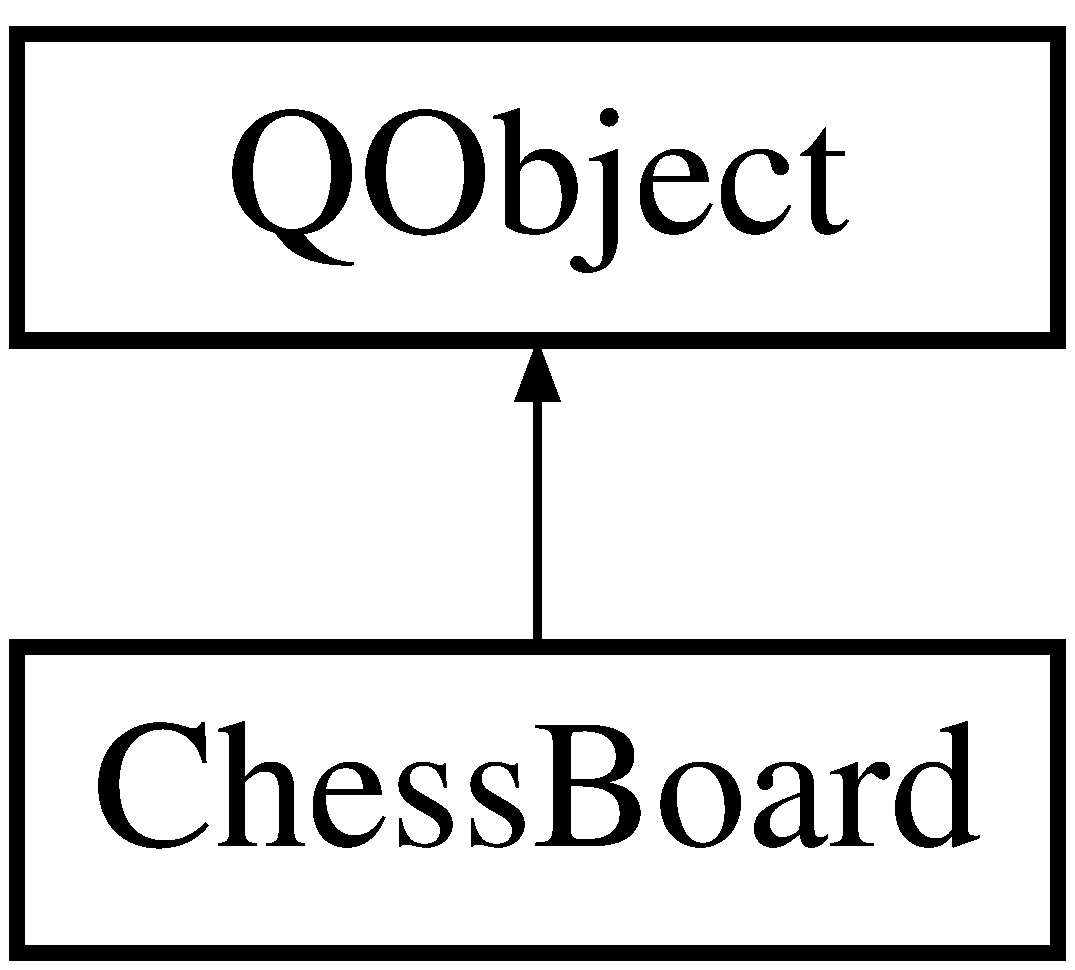
\includegraphics[height=2.000000cm]{class_chess_board}
\end{center}
\end{figure}
\subsection*{Public Member Functions}
\begin{DoxyCompactItemize}
\item 
\hyperlink{class_chess_board_aaf5e38879e16f626b94f42cb2cb2a9f2}{Chess\+Board} (Q\+Object $\ast$parent=0)
\begin{DoxyCompactList}\small\item\em Create instance. \end{DoxyCompactList}\item 
\mbox{\Hypertarget{class_chess_board_a266c0a96414a8f1605f40288a81cda60}\label{class_chess_board_a266c0a96414a8f1605f40288a81cda60}} 
void \hyperlink{class_chess_board_a266c0a96414a8f1605f40288a81cda60}{init} ()
\begin{DoxyCompactList}\small\item\em Init and clear borad. \end{DoxyCompactList}\item 
bool \hyperlink{class_chess_board_afe130ad0f67ced921f9dacf14176cb78}{insert\+Pices} (int x, int y, int type)
\begin{DoxyCompactList}\small\item\em Insert a pices. \end{DoxyCompactList}\item 
\mbox{\Hypertarget{class_chess_board_abe62b2f62c6179fb77c81b84fc17dba2}\label{class_chess_board_abe62b2f62c6179fb77c81b84fc17dba2}} 
void \hyperlink{class_chess_board_abe62b2f62c6179fb77c81b84fc17dba2}{print\+Board} ()
\begin{DoxyCompactList}\small\item\em Print the chess board status. \end{DoxyCompactList}\item 
Pices\+Pos\+List \hyperlink{class_chess_board_a385358d9aa201c8043e25aecd7dc93eb}{get\+Available\+Pos} (int board\mbox{[}4\mbox{]}\mbox{[}4\mbox{]}\mbox{[}4\mbox{]}, chess\+Pices\+Status side)
\begin{DoxyCompactList}\small\item\em Return a list of avliable pos, including pos and score. \end{DoxyCompactList}\item 
int \hyperlink{class_chess_board_a8208e18ec3b29a039ffe45249d4d9e53}{get\+Pos\+Value} (int board\mbox{[}4\mbox{]}\mbox{[}4\mbox{]}\mbox{[}4\mbox{]}, \hyperlink{struct_pices_pos}{Pices\+Pos} $\ast$pos, chess\+Pices\+Status side)
\begin{DoxyCompactList}\small\item\em Return position\textquotesingle{}s value. \end{DoxyCompactList}\item 
int \hyperlink{class_chess_board_a45115518c4f03974c31eb944ac6fa521}{get\+Flat\+Pices\+Value} (Pices\+Flat\+Data\+List flats, chess\+Pices\+Status status)
\begin{DoxyCompactList}\small\item\em Return group(flat data)\textquotesingle{}s value. \end{DoxyCompactList}\item 
int \hyperlink{class_chess_board_aae32c08142508998bedeb0907f35e62f}{get\+Side\+Score} (int board\mbox{[}4\mbox{]}\mbox{[}4\mbox{]}\mbox{[}4\mbox{]}, chess\+Pices\+Status side)
\begin{DoxyCompactList}\small\item\em Return side\textquotesingle{}s globe score. \end{DoxyCompactList}\item 
int \hyperlink{class_chess_board_a3195308e0aecff2ad8b044b7118a5a4c}{dfs} (int board\mbox{[}4\mbox{]}\mbox{[}4\mbox{]}\mbox{[}4\mbox{]}, int deep=6)
\begin{DoxyCompactList}\small\item\em Main search pridect function. \end{DoxyCompactList}\item 
int \hyperlink{class_chess_board_af1577bee7c63bad019fdda023041ad96}{find\+White\+Score\+Max\+Value} (int board\mbox{[}4\mbox{]}\mbox{[}4\mbox{]}\mbox{[}4\mbox{]}, int deep, int alpha, int beta)
\begin{DoxyCompactList}\small\item\em Search white pices\textquotesingle{} best steps. \end{DoxyCompactList}\item 
int \hyperlink{class_chess_board_ac23dc6b8a273c3e1fafb78d98e5e67d0}{find\+White\+Score\+Min\+Value} (int board\mbox{[}4\mbox{]}\mbox{[}4\mbox{]}\mbox{[}4\mbox{]}, int deep, int alpha, int beta)
\begin{DoxyCompactList}\small\item\em Search black pices\textquotesingle{} best steps. \end{DoxyCompactList}\item 
int \hyperlink{class_chess_board_abf92d3ef0baf837f8a15b8746d4e44cc}{is\+Win} (int board\mbox{[}4\mbox{]}\mbox{[}4\mbox{]}\mbox{[}4\mbox{]})
\begin{DoxyCompactList}\small\item\em Return is anyone win. \end{DoxyCompactList}\item 
Pices\+Pos\+List \hyperlink{class_chess_board_ae623e32e472e4bb21198707b9b22213f}{takeback} (int board\mbox{[}4\mbox{]}\mbox{[}4\mbox{]}\mbox{[}4\mbox{]}, int step)
\begin{DoxyCompactList}\small\item\em Take back. \end{DoxyCompactList}\end{DoxyCompactItemize}
\subsection*{Public Attributes}
\begin{DoxyCompactItemize}
\item 
int \hyperlink{class_chess_board_ab58be444056dbb531b3b2535b4054b54}{chess\+Board} \mbox{[}4\mbox{]}\mbox{[}4\mbox{]}\mbox{[}4\mbox{]}
\item 
\hyperlink{struct_pices_pos}{Pices\+Pos} \hyperlink{class_chess_board_aa03bcc987457e608a908809663085302}{white\+Target\+Pos}
\item 
\hyperlink{struct_pices_pos}{Pices\+Pos} \hyperlink{class_chess_board_a5d8e4b1cbd87ef1dd7bac6de42e375ff}{black\+Target\+Pos}
\item 
\hyperlink{struct_pices_pos}{Pices\+Pos} \hyperlink{class_chess_board_af130ebe77300106c1a79a8fd54600cd2}{target\+Pos}
\end{DoxyCompactItemize}


\subsection{Detailed Description}
Logic class. 

\subsection{Constructor \& Destructor Documentation}
\mbox{\Hypertarget{class_chess_board_aaf5e38879e16f626b94f42cb2cb2a9f2}\label{class_chess_board_aaf5e38879e16f626b94f42cb2cb2a9f2}} 
\index{Chess\+Board@{Chess\+Board}!Chess\+Board@{Chess\+Board}}
\index{Chess\+Board@{Chess\+Board}!Chess\+Board@{Chess\+Board}}
\subsubsection{\texorpdfstring{Chess\+Board()}{ChessBoard()}}
{\footnotesize\ttfamily Chess\+Board\+::\+Chess\+Board (\begin{DoxyParamCaption}\item[{Q\+Object $\ast$}]{parent = {\ttfamily 0} }\end{DoxyParamCaption})\hspace{0.3cm}{\ttfamily [explicit]}}



Create instance. 


\begin{DoxyParams}{Parameters}
{\em parent} & \\
\hline
\end{DoxyParams}


\subsection{Member Function Documentation}
\mbox{\Hypertarget{class_chess_board_a3195308e0aecff2ad8b044b7118a5a4c}\label{class_chess_board_a3195308e0aecff2ad8b044b7118a5a4c}} 
\index{Chess\+Board@{Chess\+Board}!dfs@{dfs}}
\index{dfs@{dfs}!Chess\+Board@{Chess\+Board}}
\subsubsection{\texorpdfstring{dfs()}{dfs()}}
{\footnotesize\ttfamily int Chess\+Board\+::dfs (\begin{DoxyParamCaption}\item[{int}]{board\mbox{[}4\mbox{]}\mbox{[}4\mbox{]}\mbox{[}4\mbox{]},  }\item[{int}]{deep = {\ttfamily 6} }\end{DoxyParamCaption})}



Main search pridect function. 


\begin{DoxyParams}{Parameters}
{\em board\mbox{[}$\,$\mbox{]}\mbox{[}$\,$\mbox{]}\mbox{[}$\,$\mbox{]}} & \\
\hline
{\em deep} & \\
\hline
\end{DoxyParams}
\begin{DoxyReturn}{Returns}
int 
\end{DoxyReturn}
\mbox{\Hypertarget{class_chess_board_af1577bee7c63bad019fdda023041ad96}\label{class_chess_board_af1577bee7c63bad019fdda023041ad96}} 
\index{Chess\+Board@{Chess\+Board}!find\+White\+Score\+Max\+Value@{find\+White\+Score\+Max\+Value}}
\index{find\+White\+Score\+Max\+Value@{find\+White\+Score\+Max\+Value}!Chess\+Board@{Chess\+Board}}
\subsubsection{\texorpdfstring{find\+White\+Score\+Max\+Value()}{findWhiteScoreMaxValue()}}
{\footnotesize\ttfamily int Chess\+Board\+::find\+White\+Score\+Max\+Value (\begin{DoxyParamCaption}\item[{int}]{board\mbox{[}4\mbox{]}\mbox{[}4\mbox{]}\mbox{[}4\mbox{]},  }\item[{int}]{deep,  }\item[{int}]{alpha,  }\item[{int}]{beta }\end{DoxyParamCaption})}



Search white pices\textquotesingle{} best steps. 


\begin{DoxyParams}{Parameters}
{\em board\mbox{[}$\,$\mbox{]}\mbox{[}$\,$\mbox{]}\mbox{[}$\,$\mbox{]}} & \\
\hline
{\em deep} & \\
\hline
{\em alpha} & \\
\hline
{\em beta} & \\
\hline
\end{DoxyParams}
\begin{DoxyReturn}{Returns}
int 
\end{DoxyReturn}
\mbox{\Hypertarget{class_chess_board_ac23dc6b8a273c3e1fafb78d98e5e67d0}\label{class_chess_board_ac23dc6b8a273c3e1fafb78d98e5e67d0}} 
\index{Chess\+Board@{Chess\+Board}!find\+White\+Score\+Min\+Value@{find\+White\+Score\+Min\+Value}}
\index{find\+White\+Score\+Min\+Value@{find\+White\+Score\+Min\+Value}!Chess\+Board@{Chess\+Board}}
\subsubsection{\texorpdfstring{find\+White\+Score\+Min\+Value()}{findWhiteScoreMinValue()}}
{\footnotesize\ttfamily int Chess\+Board\+::find\+White\+Score\+Min\+Value (\begin{DoxyParamCaption}\item[{int}]{board\mbox{[}4\mbox{]}\mbox{[}4\mbox{]}\mbox{[}4\mbox{]},  }\item[{int}]{deep,  }\item[{int}]{alpha,  }\item[{int}]{beta }\end{DoxyParamCaption})}



Search black pices\textquotesingle{} best steps. 


\begin{DoxyParams}{Parameters}
{\em board\mbox{[}$\,$\mbox{]}\mbox{[}$\,$\mbox{]}\mbox{[}$\,$\mbox{]}} & \\
\hline
{\em deep} & \\
\hline
{\em alpha} & \\
\hline
{\em beta} & \\
\hline
\end{DoxyParams}
\begin{DoxyReturn}{Returns}
int 
\end{DoxyReturn}
\mbox{\Hypertarget{class_chess_board_a385358d9aa201c8043e25aecd7dc93eb}\label{class_chess_board_a385358d9aa201c8043e25aecd7dc93eb}} 
\index{Chess\+Board@{Chess\+Board}!get\+Available\+Pos@{get\+Available\+Pos}}
\index{get\+Available\+Pos@{get\+Available\+Pos}!Chess\+Board@{Chess\+Board}}
\subsubsection{\texorpdfstring{get\+Available\+Pos()}{getAvailablePos()}}
{\footnotesize\ttfamily Pices\+Pos\+List Chess\+Board\+::get\+Available\+Pos (\begin{DoxyParamCaption}\item[{int}]{board\mbox{[}4\mbox{]}\mbox{[}4\mbox{]}\mbox{[}4\mbox{]},  }\item[{chess\+Pices\+Status}]{side }\end{DoxyParamCaption})}



Return a list of avliable pos, including pos and score. 


\begin{DoxyParams}{Parameters}
{\em board\mbox{[}$\,$\mbox{]}\mbox{[}$\,$\mbox{]}\mbox{[}$\,$\mbox{]}} & \\
\hline
{\em side} & \\
\hline
\end{DoxyParams}
\begin{DoxyReturn}{Returns}
Pices\+Pos\+List 
\end{DoxyReturn}
\mbox{\Hypertarget{class_chess_board_a45115518c4f03974c31eb944ac6fa521}\label{class_chess_board_a45115518c4f03974c31eb944ac6fa521}} 
\index{Chess\+Board@{Chess\+Board}!get\+Flat\+Pices\+Value@{get\+Flat\+Pices\+Value}}
\index{get\+Flat\+Pices\+Value@{get\+Flat\+Pices\+Value}!Chess\+Board@{Chess\+Board}}
\subsubsection{\texorpdfstring{get\+Flat\+Pices\+Value()}{getFlatPicesValue()}}
{\footnotesize\ttfamily int Chess\+Board\+::get\+Flat\+Pices\+Value (\begin{DoxyParamCaption}\item[{Pices\+Flat\+Data\+List}]{flats,  }\item[{chess\+Pices\+Status}]{status }\end{DoxyParamCaption})}



Return group(flat data)\textquotesingle{}s value. 


\begin{DoxyParams}{Parameters}
{\em flats} & \\
\hline
{\em status} & \\
\hline
\end{DoxyParams}
\begin{DoxyReturn}{Returns}
int 
\end{DoxyReturn}
\mbox{\Hypertarget{class_chess_board_a8208e18ec3b29a039ffe45249d4d9e53}\label{class_chess_board_a8208e18ec3b29a039ffe45249d4d9e53}} 
\index{Chess\+Board@{Chess\+Board}!get\+Pos\+Value@{get\+Pos\+Value}}
\index{get\+Pos\+Value@{get\+Pos\+Value}!Chess\+Board@{Chess\+Board}}
\subsubsection{\texorpdfstring{get\+Pos\+Value()}{getPosValue()}}
{\footnotesize\ttfamily int Chess\+Board\+::get\+Pos\+Value (\begin{DoxyParamCaption}\item[{int}]{board\mbox{[}4\mbox{]}\mbox{[}4\mbox{]}\mbox{[}4\mbox{]},  }\item[{\hyperlink{struct_pices_pos}{Pices\+Pos} $\ast$}]{pos,  }\item[{chess\+Pices\+Status}]{side }\end{DoxyParamCaption})}



Return position\textquotesingle{}s value. 


\begin{DoxyParams}{Parameters}
{\em board\mbox{[}$\,$\mbox{]}\mbox{[}$\,$\mbox{]}\mbox{[}$\,$\mbox{]}} & \\
\hline
{\em pos} & \\
\hline
{\em side} & \\
\hline
\end{DoxyParams}
\begin{DoxyReturn}{Returns}
int 
\end{DoxyReturn}
\mbox{\Hypertarget{class_chess_board_aae32c08142508998bedeb0907f35e62f}\label{class_chess_board_aae32c08142508998bedeb0907f35e62f}} 
\index{Chess\+Board@{Chess\+Board}!get\+Side\+Score@{get\+Side\+Score}}
\index{get\+Side\+Score@{get\+Side\+Score}!Chess\+Board@{Chess\+Board}}
\subsubsection{\texorpdfstring{get\+Side\+Score()}{getSideScore()}}
{\footnotesize\ttfamily int Chess\+Board\+::get\+Side\+Score (\begin{DoxyParamCaption}\item[{int}]{board\mbox{[}4\mbox{]}\mbox{[}4\mbox{]}\mbox{[}4\mbox{]},  }\item[{chess\+Pices\+Status}]{side }\end{DoxyParamCaption})}



Return side\textquotesingle{}s globe score. 


\begin{DoxyParams}{Parameters}
{\em board\mbox{[}$\,$\mbox{]}\mbox{[}$\,$\mbox{]}\mbox{[}$\,$\mbox{]}} & \\
\hline
{\em side} & \\
\hline
\end{DoxyParams}
\begin{DoxyReturn}{Returns}
int 
\end{DoxyReturn}
\mbox{\Hypertarget{class_chess_board_afe130ad0f67ced921f9dacf14176cb78}\label{class_chess_board_afe130ad0f67ced921f9dacf14176cb78}} 
\index{Chess\+Board@{Chess\+Board}!insert\+Pices@{insert\+Pices}}
\index{insert\+Pices@{insert\+Pices}!Chess\+Board@{Chess\+Board}}
\subsubsection{\texorpdfstring{insert\+Pices()}{insertPices()}}
{\footnotesize\ttfamily bool Chess\+Board\+::insert\+Pices (\begin{DoxyParamCaption}\item[{int}]{x,  }\item[{int}]{y,  }\item[{int}]{type }\end{DoxyParamCaption})}



Insert a pices. 


\begin{DoxyParams}{Parameters}
{\em x} & \\
\hline
{\em y} & \\
\hline
{\em type} & \\
\hline
\end{DoxyParams}
\begin{DoxyReturn}{Returns}
The pos is a valid pos or not. 
\end{DoxyReturn}
\mbox{\Hypertarget{class_chess_board_abf92d3ef0baf837f8a15b8746d4e44cc}\label{class_chess_board_abf92d3ef0baf837f8a15b8746d4e44cc}} 
\index{Chess\+Board@{Chess\+Board}!is\+Win@{is\+Win}}
\index{is\+Win@{is\+Win}!Chess\+Board@{Chess\+Board}}
\subsubsection{\texorpdfstring{is\+Win()}{isWin()}}
{\footnotesize\ttfamily int Chess\+Board\+::is\+Win (\begin{DoxyParamCaption}\item[{int}]{board\mbox{[}4\mbox{]}\mbox{[}4\mbox{]}\mbox{[}4\mbox{]} }\end{DoxyParamCaption})}



Return is anyone win. 


\begin{DoxyParams}{Parameters}
{\em board\mbox{[}$\,$\mbox{]}\mbox{[}$\,$\mbox{]}\mbox{[}$\,$\mbox{]}} & \\
\hline
\end{DoxyParams}
\begin{DoxyReturn}{Returns}
int 
\end{DoxyReturn}
\mbox{\Hypertarget{class_chess_board_ae623e32e472e4bb21198707b9b22213f}\label{class_chess_board_ae623e32e472e4bb21198707b9b22213f}} 
\index{Chess\+Board@{Chess\+Board}!takeback@{takeback}}
\index{takeback@{takeback}!Chess\+Board@{Chess\+Board}}
\subsubsection{\texorpdfstring{takeback()}{takeback()}}
{\footnotesize\ttfamily Pices\+Pos\+List Chess\+Board\+::takeback (\begin{DoxyParamCaption}\item[{int}]{board\mbox{[}4\mbox{]}\mbox{[}4\mbox{]}\mbox{[}4\mbox{]},  }\item[{int}]{step }\end{DoxyParamCaption})}



Take back. 


\begin{DoxyParams}{Parameters}
{\em board\mbox{[}$\,$\mbox{]}\mbox{[}$\,$\mbox{]}\mbox{[}$\,$\mbox{]}} & \\
\hline
{\em step} & \\
\hline
\end{DoxyParams}
\begin{DoxyReturn}{Returns}
Pices\+Pos\+List 
\end{DoxyReturn}


\subsection{Member Data Documentation}
\mbox{\Hypertarget{class_chess_board_a5d8e4b1cbd87ef1dd7bac6de42e375ff}\label{class_chess_board_a5d8e4b1cbd87ef1dd7bac6de42e375ff}} 
\index{Chess\+Board@{Chess\+Board}!black\+Target\+Pos@{black\+Target\+Pos}}
\index{black\+Target\+Pos@{black\+Target\+Pos}!Chess\+Board@{Chess\+Board}}
\subsubsection{\texorpdfstring{black\+Target\+Pos}{blackTargetPos}}
{\footnotesize\ttfamily \hyperlink{struct_pices_pos}{Pices\+Pos} Chess\+Board\+::black\+Target\+Pos}

Pridect black pices target pos \mbox{\Hypertarget{class_chess_board_ab58be444056dbb531b3b2535b4054b54}\label{class_chess_board_ab58be444056dbb531b3b2535b4054b54}} 
\index{Chess\+Board@{Chess\+Board}!chess\+Board@{chess\+Board}}
\index{chess\+Board@{chess\+Board}!Chess\+Board@{Chess\+Board}}
\subsubsection{\texorpdfstring{chess\+Board}{chessBoard}}
{\footnotesize\ttfamily int Chess\+Board\+::chess\+Board\mbox{[}4\mbox{]}\mbox{[}4\mbox{]}\mbox{[}4\mbox{]}}

Chess Board x,y,z \mbox{\Hypertarget{class_chess_board_af130ebe77300106c1a79a8fd54600cd2}\label{class_chess_board_af130ebe77300106c1a79a8fd54600cd2}} 
\index{Chess\+Board@{Chess\+Board}!target\+Pos@{target\+Pos}}
\index{target\+Pos@{target\+Pos}!Chess\+Board@{Chess\+Board}}
\subsubsection{\texorpdfstring{target\+Pos}{targetPos}}
{\footnotesize\ttfamily \hyperlink{struct_pices_pos}{Pices\+Pos} Chess\+Board\+::target\+Pos}

Result pos, this result is after compire between attach or defence \mbox{\Hypertarget{class_chess_board_aa03bcc987457e608a908809663085302}\label{class_chess_board_aa03bcc987457e608a908809663085302}} 
\index{Chess\+Board@{Chess\+Board}!white\+Target\+Pos@{white\+Target\+Pos}}
\index{white\+Target\+Pos@{white\+Target\+Pos}!Chess\+Board@{Chess\+Board}}
\subsubsection{\texorpdfstring{white\+Target\+Pos}{whiteTargetPos}}
{\footnotesize\ttfamily \hyperlink{struct_pices_pos}{Pices\+Pos} Chess\+Board\+::white\+Target\+Pos}

Pridect white pices target pos 

The documentation for this class was generated from the following files\+:\begin{DoxyCompactItemize}
\item 
chessboard.\+h\item 
chessboard.\+cpp\end{DoxyCompactItemize}

\hypertarget{struct_flats_data}{}\section{Flats\+Data Struct Reference}
\label{struct_flats_data}\index{Flats\+Data@{Flats\+Data}}


Flat data group.  




{\ttfamily \#include $<$chessboard.\+h$>$}

\subsection*{Public Attributes}
\begin{DoxyCompactItemize}
\item 
int \hyperlink{struct_flats_data_ab05a4bc13a98636cf93edfc965afb462}{a}
\item 
int \hyperlink{struct_flats_data_aaca73684b48fe7211c676b721bc3ba9d}{b}
\item 
int \hyperlink{struct_flats_data_a19152c81d88747bd221d1bd2e2a01077}{c}
\item 
int \hyperlink{struct_flats_data_a2244298a5ff35dcd06d54b283b485e35}{d}
\end{DoxyCompactItemize}


\subsection{Detailed Description}
Flat data group. 

\subsection{Member Data Documentation}
\mbox{\Hypertarget{struct_flats_data_ab05a4bc13a98636cf93edfc965afb462}\label{struct_flats_data_ab05a4bc13a98636cf93edfc965afb462}} 
\index{Flats\+Data@{Flats\+Data}!a@{a}}
\index{a@{a}!Flats\+Data@{Flats\+Data}}
\subsubsection{\texorpdfstring{a}{a}}
{\footnotesize\ttfamily int Flats\+Data\+::a}

T\+O\+DO\+: describe \mbox{\Hypertarget{struct_flats_data_aaca73684b48fe7211c676b721bc3ba9d}\label{struct_flats_data_aaca73684b48fe7211c676b721bc3ba9d}} 
\index{Flats\+Data@{Flats\+Data}!b@{b}}
\index{b@{b}!Flats\+Data@{Flats\+Data}}
\subsubsection{\texorpdfstring{b}{b}}
{\footnotesize\ttfamily int Flats\+Data\+::b}

T\+O\+DO\+: describe \mbox{\Hypertarget{struct_flats_data_a19152c81d88747bd221d1bd2e2a01077}\label{struct_flats_data_a19152c81d88747bd221d1bd2e2a01077}} 
\index{Flats\+Data@{Flats\+Data}!c@{c}}
\index{c@{c}!Flats\+Data@{Flats\+Data}}
\subsubsection{\texorpdfstring{c}{c}}
{\footnotesize\ttfamily int Flats\+Data\+::c}

T\+O\+DO\+: describe \mbox{\Hypertarget{struct_flats_data_a2244298a5ff35dcd06d54b283b485e35}\label{struct_flats_data_a2244298a5ff35dcd06d54b283b485e35}} 
\index{Flats\+Data@{Flats\+Data}!d@{d}}
\index{d@{d}!Flats\+Data@{Flats\+Data}}
\subsubsection{\texorpdfstring{d}{d}}
{\footnotesize\ttfamily int Flats\+Data\+::d}

T\+O\+DO\+: describe 

The documentation for this struct was generated from the following file\+:\begin{DoxyCompactItemize}
\item 
chessboard.\+h\end{DoxyCompactItemize}

\hypertarget{class_my_event_receiver}{}\section{My\+Event\+Receiver Class Reference}
\label{class_my_event_receiver}\index{My\+Event\+Receiver@{My\+Event\+Receiver}}


Main UI handler.  


Inheritance diagram for My\+Event\+Receiver\+:\begin{figure}[H]
\begin{center}
\leavevmode
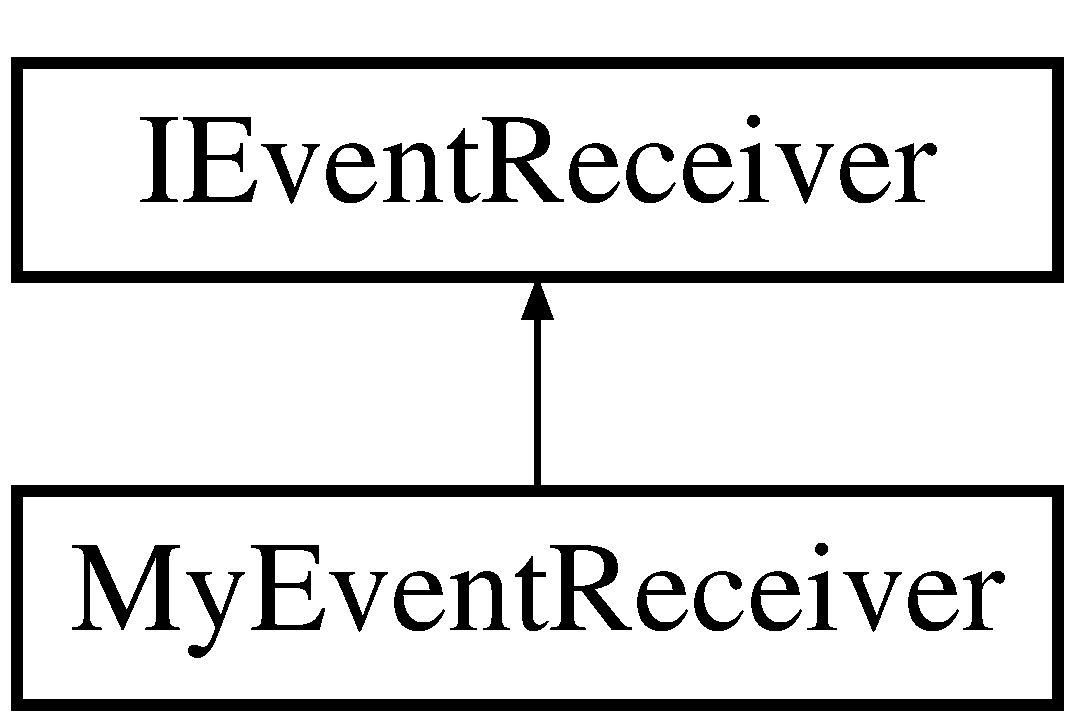
\includegraphics[height=2.000000cm]{class_my_event_receiver}
\end{center}
\end{figure}
\subsection*{Public Member Functions}
\begin{DoxyCompactItemize}
\item 
virtual bool \hyperlink{class_my_event_receiver_aea4aee9bbe18deae0c33ad4c6c32d7f1}{On\+Event} (const S\+Event \&event)
\begin{DoxyCompactList}\small\item\em On event. \end{DoxyCompactList}\item 
const \hyperlink{struct_s_mouse_state}{S\+Mouse\+State} \& \hyperlink{class_my_event_receiver_a8fb089e7c1648013762442e4676c4d91}{Get\+Mouse\+State} (void) const
\end{DoxyCompactItemize}


\subsection{Detailed Description}
Main UI handler. 

\subsection{Member Function Documentation}
\mbox{\Hypertarget{class_my_event_receiver_a8fb089e7c1648013762442e4676c4d91}\label{class_my_event_receiver_a8fb089e7c1648013762442e4676c4d91}} 
\index{My\+Event\+Receiver@{My\+Event\+Receiver}!Get\+Mouse\+State@{Get\+Mouse\+State}}
\index{Get\+Mouse\+State@{Get\+Mouse\+State}!My\+Event\+Receiver@{My\+Event\+Receiver}}
\subsubsection{\texorpdfstring{Get\+Mouse\+State()}{GetMouseState()}}
{\footnotesize\ttfamily const \hyperlink{struct_s_mouse_state}{S\+Mouse\+State}\& My\+Event\+Receiver\+::\+Get\+Mouse\+State (\begin{DoxyParamCaption}\item[{void}]{ }\end{DoxyParamCaption}) const\hspace{0.3cm}{\ttfamily [inline]}}

\begin{DoxyReturn}{Returns}
const \hyperlink{struct_s_mouse_state}{S\+Mouse\+State} 
\end{DoxyReturn}
\mbox{\Hypertarget{class_my_event_receiver_aea4aee9bbe18deae0c33ad4c6c32d7f1}\label{class_my_event_receiver_aea4aee9bbe18deae0c33ad4c6c32d7f1}} 
\index{My\+Event\+Receiver@{My\+Event\+Receiver}!On\+Event@{On\+Event}}
\index{On\+Event@{On\+Event}!My\+Event\+Receiver@{My\+Event\+Receiver}}
\subsubsection{\texorpdfstring{On\+Event()}{OnEvent()}}
{\footnotesize\ttfamily virtual bool My\+Event\+Receiver\+::\+On\+Event (\begin{DoxyParamCaption}\item[{const S\+Event \&}]{event }\end{DoxyParamCaption})\hspace{0.3cm}{\ttfamily [inline]}, {\ttfamily [virtual]}}



On event. 


\begin{DoxyParams}{Parameters}
{\em event} & \\
\hline
\end{DoxyParams}
\begin{DoxyReturn}{Returns}
bool 
\end{DoxyReturn}


The documentation for this class was generated from the following file\+:\begin{DoxyCompactItemize}
\item 
main.\+cpp\end{DoxyCompactItemize}

\hypertarget{struct_pices_pos}{}\section{Pices\+Pos Struct Reference}
\label{struct_pices_pos}\index{Pices\+Pos@{Pices\+Pos}}


Single pices status.  




{\ttfamily \#include $<$chessboard.\+h$>$}

\subsection*{Public Attributes}
\begin{DoxyCompactItemize}
\item 
int \hyperlink{struct_pices_pos_acb1106796cffe0be268d0520a204656d}{x}
\item 
int \hyperlink{struct_pices_pos_a72146b86f290ee233d93a483d07f1922}{y}
\item 
int \hyperlink{struct_pices_pos_a195acdcf09f1c447e48975aed219f5be}{z}
\item 
chess\+Pices\+Status \hyperlink{struct_pices_pos_a297ffb0e8b5dd50be9fb6cf6af22d9b7}{type}
\item 
int \hyperlink{struct_pices_pos_aafd38b1dbfa288fdafc2e7565238560f}{value}
\end{DoxyCompactItemize}


\subsection{Detailed Description}
Single pices status. 

\subsection{Member Data Documentation}
\mbox{\Hypertarget{struct_pices_pos_a297ffb0e8b5dd50be9fb6cf6af22d9b7}\label{struct_pices_pos_a297ffb0e8b5dd50be9fb6cf6af22d9b7}} 
\index{Pices\+Pos@{Pices\+Pos}!type@{type}}
\index{type@{type}!Pices\+Pos@{Pices\+Pos}}
\subsubsection{\texorpdfstring{type}{type}}
{\footnotesize\ttfamily chess\+Pices\+Status Pices\+Pos\+::type}

Pices Status \mbox{\Hypertarget{struct_pices_pos_aafd38b1dbfa288fdafc2e7565238560f}\label{struct_pices_pos_aafd38b1dbfa288fdafc2e7565238560f}} 
\index{Pices\+Pos@{Pices\+Pos}!value@{value}}
\index{value@{value}!Pices\+Pos@{Pices\+Pos}}
\subsubsection{\texorpdfstring{value}{value}}
{\footnotesize\ttfamily int Pices\+Pos\+::value}

Position value \mbox{\Hypertarget{struct_pices_pos_acb1106796cffe0be268d0520a204656d}\label{struct_pices_pos_acb1106796cffe0be268d0520a204656d}} 
\index{Pices\+Pos@{Pices\+Pos}!x@{x}}
\index{x@{x}!Pices\+Pos@{Pices\+Pos}}
\subsubsection{\texorpdfstring{x}{x}}
{\footnotesize\ttfamily int Pices\+Pos\+::x}

X pos \mbox{\Hypertarget{struct_pices_pos_a72146b86f290ee233d93a483d07f1922}\label{struct_pices_pos_a72146b86f290ee233d93a483d07f1922}} 
\index{Pices\+Pos@{Pices\+Pos}!y@{y}}
\index{y@{y}!Pices\+Pos@{Pices\+Pos}}
\subsubsection{\texorpdfstring{y}{y}}
{\footnotesize\ttfamily int Pices\+Pos\+::y}

Y pos \mbox{\Hypertarget{struct_pices_pos_a195acdcf09f1c447e48975aed219f5be}\label{struct_pices_pos_a195acdcf09f1c447e48975aed219f5be}} 
\index{Pices\+Pos@{Pices\+Pos}!z@{z}}
\index{z@{z}!Pices\+Pos@{Pices\+Pos}}
\subsubsection{\texorpdfstring{z}{z}}
{\footnotesize\ttfamily int Pices\+Pos\+::z}

z pos 

The documentation for this struct was generated from the following file\+:\begin{DoxyCompactItemize}
\item 
chessboard.\+h\end{DoxyCompactItemize}

\hypertarget{struct_s_mouse_state}{}\section{S\+Mouse\+State Struct Reference}
\label{struct_s_mouse_state}\index{S\+Mouse\+State@{S\+Mouse\+State}}


Mouse status.  


\subsection*{Public Attributes}
\begin{DoxyCompactItemize}
\item 
core\+::position2di \hyperlink{struct_s_mouse_state_a0e89a875bcf6ced1638d06c8bdf6e172}{Position}
\item 
bool \hyperlink{struct_s_mouse_state_a38522f3e2b4c04c6333a0cdfd649d52e}{Left\+Button\+Down}
\end{DoxyCompactItemize}


\subsection{Detailed Description}
Mouse status. 

\subsection{Member Data Documentation}
\mbox{\Hypertarget{struct_s_mouse_state_a38522f3e2b4c04c6333a0cdfd649d52e}\label{struct_s_mouse_state_a38522f3e2b4c04c6333a0cdfd649d52e}} 
\index{S\+Mouse\+State@{S\+Mouse\+State}!Left\+Button\+Down@{Left\+Button\+Down}}
\index{Left\+Button\+Down@{Left\+Button\+Down}!S\+Mouse\+State@{S\+Mouse\+State}}
\subsubsection{\texorpdfstring{Left\+Button\+Down}{LeftButtonDown}}
{\footnotesize\ttfamily bool S\+Mouse\+State\+::\+Left\+Button\+Down}

T\+O\+DO\+: describe \mbox{\Hypertarget{struct_s_mouse_state_a0e89a875bcf6ced1638d06c8bdf6e172}\label{struct_s_mouse_state_a0e89a875bcf6ced1638d06c8bdf6e172}} 
\index{S\+Mouse\+State@{S\+Mouse\+State}!Position@{Position}}
\index{Position@{Position}!S\+Mouse\+State@{S\+Mouse\+State}}
\subsubsection{\texorpdfstring{Position}{Position}}
{\footnotesize\ttfamily core\+::position2di S\+Mouse\+State\+::\+Position}

T\+O\+DO\+: describe 

The documentation for this struct was generated from the following file\+:\begin{DoxyCompactItemize}
\item 
main.\+cpp\end{DoxyCompactItemize}

%--- End generated contents ---

% Index
\backmatter
\newpage
\phantomsection
\clearemptydoublepage
\addcontentsline{toc}{chapter}{Index}
\printindex

\end{document}
